\newcommand{\bew}{\mathsf{Bew}}
% per scrivere eqz più velocemente
\newcommand{\eq}[1]{\begin{equation} #1 \end{equation}}
% per fare le parentesi squadrate
\newcommand{\gdnum}[1]{\ulcorner #1 \urcorner}
% per scrivere pi velocemente un'eqz e darle un label
\newcommand{\eqconnome}[2]{\begin{equation} \label{eq:#2} #1 \end{equation}}

\chapter{Macchine di Turing}

\section{Introduzione}
Intuitivamente diciamo che una funzione \`e calcolabile se esiste un insieme
finito di istruzioni che ci dica esattamente cosa dobbiamo fare, senza lasciare
nulla di sottointeso ed ambiguo. Possiamo parlare quindi di una procedura
effettiva (meccanica) proprio perch\`e la sua esecuzione deve dipendere
unicamente dagli input e dalle regole che applico (fattori come il tempo, lo
spazio, il singolo esecutore non devono influire sul risultato) e quindi
possiamo immaginare tale procedura eseguibile da una macchina ipotetica.

Pensiamo ad una macchina come ad un sistema che possiede certe abilit\`a, \`e
quindi in grado di fare certe cose. Ci concentreremo sulle procedure effettive
che potremo scrivere con una certa macchina e che tipo di funzioni potremo
rappresentare.

\section{Definizione di Macchina di Turing}
Il logico inglese Alan Turing nel suo articolo del 1936 era interessato alla
questione di cosa volesse dire calcolabile e descrisse quindi dei dispositivi
astratti conosciuti come Macchine di Turing. Prima di tutto vediamo pi\`u in
dettaglio come Turing descrive una macchina.

Turing stesso paragon\`o una macchina al comportamento di un essere umano che
sta eseguendo un calcolo.  Immaginiamo perci\'o un uomo seduto ad una scrivania
munito di carta e penna: immaginiamo quindi quest'uomo come una testina di
controllo che possa scrivere simboli di un certo alfabeto su di un ipotetico
foglio di carta che noi chiameremo nastro.

Poich\'e non \`e importante il numero di fogli a disposizione dell'uomo,
supporremo la carta come una risorsa infinita: questo si traduce nel fatto che
il nastro su cui la testina di controllo scrive sia infinito in entrambe le
direzioni.

In secondo luogo, l'uomo pu\`o ricordare ed ha memoria finita, quindi dotiamo la
testina di un numero finito di stati di memoria. Infine, la scrittura su di un
pezzo di carta comporta l'avanzamento del processo di scrittura; parallelamente
la scrittura su nastro di un simbolo comporter\`a l'avanzamento verso destra o
verso sinistra della testina medesima.

Dopo queste analogie possiamo riassumere la definizione di Macchina di Turing in
questo modo.

Una macchina di Turing (MdT) \`e definita da un \textsl{insieme di
  regole} che definiscono il comportamento della macchina su un nastro
di input-output (lettura e scrittura). Il nastro pu\`o essere
immaginato come un nastro di lunghezza infinita diviso in quadratini
dette \textsl{celle}. Ogni cella contiene un simbolo $S_i$ di un certo
alfabeto oppure \`e vuota e questo viene rappresentato dal carattere
Blank ($B$). La macchina ha una testina che si sposta lungo il nastro
iniziando dalla cella che contiene il simbolo pi\`u a sinistra e
analizzando una cella alla volta: i simboli devono essere posizionati
in celle vicine e si possono concatenare anche pi\`u input dividendoli
al pi\`u da un carattere B di Blank. I caratteri di Blank si
susseguono anche al di fuori della sequenza di simboli dati in input,
occupando tutta la lunghezza infinita del nastro.  La testina \`e
dotata di un numero finito di stati di memoria $q_i$. Lo stato ha la
funzione di un'etichetta: ad uno stato $q_i$ corrisponde un'operazione
se viene letto un simbolo $S_j$ e un'altra operazione se viene letto
il simbolo $B$. Inoltre a seconda dello stato in cui la testina si
trova, sa che simboli ha letto prima.

\begin{figure}[htbp!]
\centering
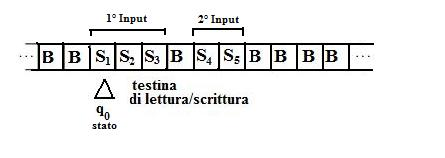
\includegraphics[scale=0.8]{img/Nastro.jpg}
\end{figure}

La macchina legge, scrive oppure cancella i simboli nelle celle del nastro
seguendo l'insieme di regole o quintuple,  che ne definiscono il comportamento.
Tali regole sono di questo tipo:

\vspace{0.3cm}
(\textsl{stato-interno-corrente}, \textsl{simbolo-letto},
\textsl{simbolo-scritto}, \textsl{prossimo-stato-interno}, \textsl{direzione}).
\vspace{0.3cm}

Quindi ad ogni passo, la macchina legge un simbolo sul nastro e in accordo al
suo \textsl{stato interno corrente}:

\begin{enumerate}
\item scrive un simbolo sul nastro
\item decide il suo prossimo stato interno, e decide se spostare la testina a
sinistra (L) o a destra (R) di una posizione.
\end{enumerate}
\vspace{0.5cm}

Diamo di seguito un esempio per queste istruzioni:

\begin{itemize}
\item La quintupla $<q_{i}S_{j}S_{k}Rq_{l}>$ indica che se la macchina
  si trova nello stato interno $q_{i}$ e legge sul nastro il simbolo
  $S_{j}$, allora lo sostituisce con $S_{k}$ e sposta la testina di
  lettura di una cella verso destra passando allo stato $q_{l}$
\item La quintupla $<q_{i}S_{j}S_{k}Lq_{l}>$ indica che se la macchina
  si trova nello stato $q_{i}$ e legge sul nastro il simbolo $S_{j}$,
  allora lo sostituisce con $S_{k}$ e sposta la testina di lettura di
  una cella verso sinistra lungo il nastro passando nello stato
  $q_{l}$.\\ Notiamo che i simboli $S_{j}$ e $S_{k}$ possono
  coincidere (cio\`e non sovrascrive nulla $<q_{i}S_{j}S_{j}Rq_{l}>$),
  cos\`i come $q_{i}$ pu\`o essere uguale a $q_{l}$ (ossia rimane
  nello stesso stato $<q_{i}S_{j}S_{j}Rq_{i}>$).
\item La scrittura del simbolo $B$ di Blank corrisponde a cancellare
  il contenuto di una cella. Ad esempio la quintupla
  $<q_{i}S_{j}BRq_{l}>$ indica che se la macchina si trova nello stato
  $q_{i}$ e legge $S_{j}$, allora cancella il simbolo mettendo il
  blank e sposta la testina di lettura di una cella verso destra
  passando allo stato $q_{l}$.
\end{itemize}

Noi tratteremo, in accordo col fatto che il nostro ``uomo anonim\`o''
non pu\`o scegliere cosa fare ma solo eseguire regole date. Diamo
quindi la seguente definizione:

\begin{defi}
Una Macchina di Turing si dice \underline{deterministica} se dato uno
stato $q_{i}$ e un simbolo $S_{j}$ c'\`e \textsl{al pi\`u} una
quintupla che inizi per $<q_{i},S_{j}...>$ cio\`e la testina
trovandosi in $q_{i}$ e leggendo $S_{j}$ non pu\`o scegliere cosa fare
ma solo eseguire l'unica istruzione corrispondente, \textsl{se c'\`e},
altrimenti significa che la macchina si arresta.
\end{defi}

Inoltre \`e possibile descrivere il nastro in ogni fase della
computazione che fa la macchina. Introduciamo quindi la seguente
definizione:

\begin{defi}
Una \underline{descrizione istantanea} $\alpha$ di una macchina di
Turing $\tau$ \`e un'espressione contenente esattamente un $q_{i}$ (lo
stato), i simboli sul nastro, e la cella in cui si trova la testina al
momento.
\end{defi}

Quindi una descrizione istantanea (ID) $\alpha$ \`e una stringa della
forma $$S_1S_2S_3.....S_{i-1}qS_{i}S_{i+1}......S_{n}$$ dove

\begin{enumerate}
\item q \`e lo stato della macchina di Turing;
\item $S_1S_2S_3.........S_{n}$ \`e la porzione non-blank del nastro;
\item La testina \`e sopra il simbolo i-esimo.
\end{enumerate}
\vspace{0.5cm}

Vediamo ora come una Macchina di Turing effettua i suoi
calcoli. Inizialmente il nastro contiene una sequenza finita di
simboli, detta \textsl{sequenza di ingresso}. Assumiamo che all'inizio
la testina della macchina $\tau$ sia posizionata sulla prima cella di
input, cio\`e sulla prima cella in cui c'\`e un simbolo e diciamo che
$\tau$ si trova nello stato $q_0$. La testina vede un simbolo $S_i$ e
allora parte: cerca tra le quintuple che forniscono le varie
istruzioni quella che comincia per $q_0$ e ha come secondo elemento il
simbolo letto, del tipo $<q_0,S_i..>$. A questo punto vede quale
istruzione deve eseguire (se sovrascrivere un altro simbolo o se
cancellare), in quale direzione andare e in quale stato portarsi, e
cos\`i via. Se non c'\`e una tale quintupla, la macchina si arresta.

Osserviamo che Turing propose l'idea di tale macchina che fosse capace
di eseguire ogni tipo di calcolo su numeri e simboli. Noi per
semplicit\`a ci riconduciamo a calcoli su numeri naturali e vedremo
che ci possiamo ridurre a considerare un alfabeto costituito
unicamente dai simboli 1 e B: $$\Sigma=\left\{1,B\right\}$$ e quindi
con tale alfabeto riusciremo a rappresentare tutti i numeri
naturali. Notiamo infatti che \`e del tutto equivalente considerare un
alfabeto con un simbolo o con n simboli ed i calcolatori, essendo
rappresentazioni di Macchine di Turing ed usando l'alfabeto binario lo
confermano.

Introduciamo ora una notazione che ci permetter\`a di rappresentare i
numeri naturali e quindi gli input da dare alle macchine (compreso lo
0). Per come abbiamo definito la macchina di Turing, risulta che
abbiamo a disposizione l'unico simbolo di input $1$ per rappresentare
ogni naturale o n-upla di naturali che siano nel dominio di una
funzione.

\begin{itemize}
\item preso un numero $n\in {N}$, ad esso associamo un'espressione
$$\overline{n}=1^{n+1}=\underbrace{11...1}_{n+1\ volte}\quad\mbox{.}$$
  Ad esempio $\overline{3}=1111$.
\item in maniera del tutto analoga, a una k-tupla $(n_{1}...n_{k})$ di
  interi non negativi associamo l'espressione
  $\overline{(n_{1}...n_{k})}=\overline{n_{1}}B...B\overline{n_{k}}$. Per
  esempio $$\overline{(1,4,0)}=\overline{1}B\overline{4}B\overline{0}=
  11B11111B1\quad\mbox {.}$$ In questo caso si vede come si procede
  per separare gli input, cio\`e inserendo un $B$.
\end{itemize}

Se invece con questa notazione abbiamo rappresentato nel nastro un
determinato numero indichiamo con $<\overline{n}>$ il numero naturale
da esso rappresentato, ossia $<\overline{n}>=n$.\\ Quindi gli input
che compariranno nella sequenza d'ingresso sono della forma
$$...BB\overline{n_{1}}B\overline{n_{2}}B...B\overline{n_{k}}BB...$$
dove $\overline{n_1},...,\overline{n_k}$ sono i numeri naturali nella
notazione data sopra. Converremo che ogni blocco rappresentante un
argomento \`e separato dagli altri da un solo $B$; in questo modo la
macchina sa dove inizia e termina l'input (se si incontrano due blank
consecutivi, la testina non \`e pi\`u collocata su una delle celle di
input).  La macchina di Turing su un dato input produce un output. Noi
accetteremo output della forma $$...BB\overline{n_r}BB...$$ ove
$\overline{n_r}$ \`e il risultato della computazione. Dunque in output
avremo il nastro contenente un blocco unico contenente tanti $1$
quanti sono necessari per rappresentare il risultato, in modo tale che
anche in questo caso la macchina sa dove comincia e finisce l'output,
e quindi si noti che, una volta calcolata la soluzione, sar\`a
necessario anche cancellare gli input.

\section{Varianti della Macchina di Turing}
Ci sono molteplici varianti della macchina di Turing e seppur non
entrando qui nel dettaglio si pu\`o mostrare che queste hanno la
stessa portata computazionale della macchina di Turing che abbiamo
definito all'inizio.
\begin{itemize}
\item Macchina di Turing Multinastro: invece di esservi un singolo
  nastro, vi sono k nastri indipendenti e k testine di
  lettura-scrittura, una per ogni nastro.
\item Macchina di Turing con movimento arbitrario della testina di
  lettura: si pu\`o modificare la definizione di una macchina di
  Turing in modo che la testina di lettura si possa spostare ogni
  volta di un numero arbitrario di celle
\item Macchina di Turing con nastro bidimensionale: la macchina opera
  su un nastro bidimensionale, e sono permessi spostamenti verso
  sinistra, destra, l'alto, il basso.
\item Macchina di Turing non deterministica: si distingue da quella
  deterministica definita in precedenza per il fatto che, in presenza
  di un determinato stato e di un determinato carattere letto, essa
  permette la presenza di pi\`u quintuple che iniziano con quello
  stato e quel carattere letto.
\end{itemize}


\chapter{Macchine di Turing e Funzioni Calcolabili}

\section{Cosa pu\`o Essere Calcolato}

Le macchine di Turing sono strumenti molto potenti. Per una grande
quantit\`a di problemi di calcolabilit\`a, \`e possibile costruire una
macchina di Turing che sia in grado di eseguire il calcolo
desiderato. Per esempio, abbiamo visto che \`e possibile ideare una
macchina di Turing per eseguire le operazioni aritmetiche di base sui
numeri naturali.

\subsection{Numeri Calcolabili}

Il lavoro originale di Turing trattava i numeri calcolabili. Un numero
si dice Turing-calcolabile se esiste una macchina di Turing che inizia
la computazione su un nastro vuoto e calcola un numero arbitrario, con
una certa approssimazione. Le macchine di Turing possono calcolare
tutti i numeri algebrici (radici di equazioni con coefficienti
algebrici) e molte costanti matematiche, come ad esempio $\textit{e}$
(costante di Nepero) e $\pi$.

\subsection{Funzioni Calcolabili}

Come abbiamo visto in precedenza, le macchine di Turing possono fare
molto pi\`u che calcolare semplici numeri. Tra le altre cose possono
calcolare funzioni numeriche del tipo $f:N^{n}->N$, come ad esempio si
possono scrivere macchine per calcolare la somma, la moltiplicazione,
la sottrazione tra naturali, l'esponenziale, il fattoriale e molte
altre.

Usando una convenzione per rappresentare i simboli di verit\`a TRUE e
FALSE, rappresentando, per esempio, il valore TRUE come una sequenza
di due ``1'' e il valore FALSE come un singolo ``1'', si possono
trattare anche funzioni binarie, ovvero del tipo
$f:N^{n}->\{0,1\}$. Con tali funzioni \`e possibile calcolare la
funzione caratteristica di un predicato. E', inoltre, possibile
combinare i risultati di tali funzioni con gli usuali operatori
booleani: AND, NOT, OR e in aggiunta IF-THEN-ELSE.

Difatti, le funzioni Turing-calcolabili coincidono con le funzioni
ricorsive, di cui tratteremo pi\`u avanti.

\subsection{Macchina di Turing Universale}

Il pi\`u importante e suggestivo risultato del lavoro di Turing
riguarda il fatto che, per come sono state definite le macchine di
Turing, \`e possibile definire la \textit{Macchina di Turing
  Universale} (UTM).

In teoria della computazione si dice macchina di Turing Universale
$T_U$ una macchina di Turing capace di simulare le evoluzioni di ogni
macchina di Turing. Tale macchina ha permesso di dare una risposta
negativa al problema della decidibilit\`a posto da David Hilbert nel
1928. Brevemente, il problema posto da Hilbert riguarda la
possibilit\`a o meno di poter definire un metodo matematico o un
processo per decidere tutti i possibili problemi matematici.

Essenzialmente la UTM \`e in grado di simulare il comportamento di
qualunque macchina di Turing (compresa se stessa!). Un modo per
pensare alla UTM potrebbe essere quello di immaginarla come un
interprete di un linguaggio di programmazione. Quando all'interprete
(concretamente \`e esso stesso un programma) viene dato in input un
programma, questo comincia ad eseguire le istruzioni del programma
dato e, quindi, si comporta proprio come se fosse lo stesso programma,
dato in input, ad essere eseguito.

La macchina di Turing Universale richiede in input una coppia di
numeri naturali (n,m), dove il primo \`e un indice che identifica una
specifica macchina di Turing $T_n$ (in grado di computare una data
funzione f). Mentre, il secondo indice rappresenta l'input sul quale
eseguire la macchina $T_n$.

Per poter definire una macchina del tipo descritto, \`e prima
necessario ideare un modo per rappresentare una macchina di Turing sul
nastro della UTM. E' possibile associare in modo effettivo ad ogni
macchina di Turing un numero naturale che la identifichi
univocamente. L'idea \`e quella di avere una funzione, preferibilmente
biunivoca, che mappi l'insieme delle macchine di Turing, diciamo T,
nell'insieme dei numeri naturali $f:T->N$. A tale scopo, tenendo
presente che le macchine di Turnig sono definite da una quintupla, si
pu\`o prima definire una codifica per i singoli elementi di una
quintupla e in seguito per ogni possibile quintupla. Esistono molti
modi possibili per ottenere questa codifica effettiva. Il paragrafo
\ref{codeffettiva} che segue mostra a titolo di esempio una di queste
possibili codifiche.

L'esecuzione della macchina universale $T_U(n,m)$ corrisponde quindi
ad eseguire la macchina $T_n(m)$.

\begin{center}
$T_U(n,m) = T_n(m)$
\end{center}

\vspace{10pt}

La macchina $T_U$ opera con un nastro che inizialmente in una sua
prima sezione contiene la codifica delle istruzioni della macchina
$T_n$ seguita, dopo un demarcatore particolare bene individuabile,
dallo stesso input m.

E' interesante osservare che la macchina di Turing Universale \`e in
grado di simulare anche la propria evoluzione mentre procede a
simulare una qualsiasi macchina $T$.

I computer programmabili sono effettivamente delle macchine di Turing
universali, poich\`e sono in grado di simulare l'esecuzione di ogni
macchina di Turing (se vengono intese come algoritmi che calcolano
funzioni) tramite l'esecuzione di un programma, che pu\`o essere visto
come un processo di calcolo da eseguire.

\subsection{Codifica Effettiva delle Macchine di Turing}\label{codeffettiva}

Di seguito viene riportato un'esempio di codifica effettiva per le
macchine di Turing. Con tale codifica \`e possibile rappresentare una
qualunque macchina di Turing sul nastro della macchina di Turing
universale.\\

Ogni quintupla nella definizione di una macchina sar\`a codificata
come una sequenza di cinque blocchi di ``1'', separati da un singolo
``0''.
\begin{enumerate}
  \item Il primo blocco di ``1'' sar\`a la codifica del numero dello
    stato corrente, usando la convezione sopra definita per la
    rappresentazione dei numeri naturali sul nastro (n+1 ``1''
    rappresentano il numero n).
  \item Il secondo blocco di ``1'' sar\`a la codifica del simbolo
    corrente (simbolo che si trova sotto la testina). La codifica del
    simbolo corrente dipende dall'alfabeto e dalla notazione per i
    caratteri usata.``1''
  \item Il terzo blocco di ``1'' sar\`a la codifica dell'eventuale
    simbolo da scrivere in posizione sul nastro sottostante la
    testina.
  \item Il quarto elemento rappresenter\`a l'azione che deve essere
    eseguita dalla testina, e ci sono tre possibilit\`a: con un blocco
    di un solo ``1'' si rappresanta lo spostamento nullo, con un
    blocco di due ``1'' lo spostamento a sinistra (L) e con tre ``1''
    lo spostamento a destra (R).
  \item Infine, il quinto elemento della tuple rappresenter\`a il
    numero del nuovo stato in cui la macchina si trover\`a dopo
    l'esecuzione dell'azione richiesta, rappresentato anche esso
    mediante la notazione unaria.
\end{enumerate}

Per codicifare, in fine, l'intera macchina, basta semplicemente
scrivere sul nastro tutte le tuple che caratterizzano la macchina,
separate tra loro da un carattere di \textit{Blank}.

Se si utilizza il carattere ``0'' al posto del carattere
\textit{Blank}, si ottiene una sequenza di ``0'' e di ``1''. Tale
sequenza pu\`o essere interpretata come un numero naturale espresso in
rappresetntazione binaria. Se tale numero viene espresso con la
notazione $\overline{n}=1^{n+1}$, risulta effettivamente possibile
dare in input alla macchina di Turing universale una coppia di numeri
naturali espressi secondo questa notazione.


\section{Cosa non pu\`o Essere Calcolato}
Un altro sorprendente risultato presentato dall'articolo di Turing del
1936 riguarda l'esistenza di problemi ben definiti che non possono
essere risolti da nessuna procedura computazionale. Se questi problemi
sono formulati come formule, possiamo riferirci a queste funzioni come
funzioni non calcolabili; se questi problemi vengono espressi come
predicati, si dice problemi indecidibili. Usando il concetto della
macchina astratta di turing, possiamo dire che una funzione non \`e
calcolabile se non esistono macchine di Turing che sono in grado di
calcolare tale funzione.

Per mostrare l'esitenza di funzioni non calcolabili dalle macchine di
Turing bisogna ragionare sulla cardinalit\`a dell'insieme delle
macchine di Turing e confrontarla con la cardinalit\`a dell'insieme
delle funzioni del tipo $f:N->N$ (con uno sforzo minimo ci si pu\`o
portare al caso pi\`u generale di funzioni $f:N^n->N$).

\begin{center}
$F = \{ f | f \textrm{ \`e una funzione del tipo } f:N->N \}.$
\end{center}

\vspace{10pt}

\begin{center}
$T = \{ t | t \textrm{ \`e una macchina di Turing} \}.$
\end{center}

\vspace{10pt}

Poich\`e \`e possibile, come mostrato in precedenza, costruire una
codifica effettiva delle macchine di Turing, cio\`e costruire una
funzione che associ ad ogni TM un numero naturale unico, l'insieme
delle TM \`e enumerabile, ovvero la sua cardinalit\`a \`e pari a $|N|$
(cardinalit\`a dei numeri naturali). Tuttavia, l'insieme di tutte le
funzioni $f:N->N$ \`e dimostrato non essere enumerabile. Per questo
motivo, possiamo concludere che tutte le macchine di Turing sono in
grado di calcolare solo un sottoinsieme di tutte le funzioni
definibili.

Ci sono molti problemi legati ai programmi che si possono dimostrare
non decidibili. Poich\`e le macchine di Turing sono molto semplici se
comparate con i computer come uso pratico, risulta concettualmente
pi\`u facile provare l'impossobilit\`a di alcuni risultati per le
macchine di Turing. Dando un definizione formale di non banale per una
propriet\`a, H.G. Rice riusc\`i, addirittura, a dimostrare il seguente
teorema:

\begin{thm}
Ogni propriet\`a non banale dei programmi \`e indecidibile.
\end{thm}

E' da notare che dimostrando che un problema \`e non decidibile, non
significa che non pu\`o essere deciso solo in alcuni casi, bens\`i che
\`e impossibile costruire una soluzione \textit{per ogni} possibile
input.



%%%%%%%%%%%%%%%%%%%%%%%%%%%%%%%%%%%%%%%%%%%%%%%%%ESEMPI%%%%%%%%%%%%%%%%%%%%%%%%%%%%%%%%%

\chapter{Macchine di Turing: Esempi}


\section{Esempi di Macchine di Turing}
Diamo ora qualche esempio di semplici macchine di Turing.\\

\begin{itemize}
\item Sia $\Sigma=\left\{0,1\right\}$ l'alfabeto di simboli in
  input. \\\underline{Scopo della macchina:} data una stringa di 0 e 1
  scambia le occorrenze di 1 con 0 e viceversa, riposizionandosi sulla
  cella precedente a quella iniziale.\\ \underline{Passi:} leggere i
  simboli sul nastro e ogni volta che si trova 1 si scrive 0 e
  viceversa. Quando la sequenza di 0 e 1 è finita la testina torna
  sulla cella precedente alla prima significativa.\\

Nastro in input:$$...BB100101BB....$$\\

Sequenza di quintuple:
\begin{eqnarray*}
&<q_0,0,1,R,q_0>&\\
&<q_0,1,0,R,q_0>&\mbox{(scambia 0 e 1)}\\
&<q_0,B,B,L,q_1>&\\
&<q_1,0,0,L,q_1>&\\
&<q_1,1,1,L,q_1>&\mbox{(si riposiziona sulla cella precedente alla prima significativa)}\\
\end{eqnarray*}
Quindi la macchina di Turing per la sequenza di ingresso $...BB100101BB....$ esegue la seguente computazione:
\begin{eqnarray*}
&...BBq_0100101BB...\\
&...BB0q_000101BB...\\
&...BB01q_00101BB...\\
&...BB011q_0101BB...\\
&...BB0110q_001BB...\\
&...BB01101q_01BB...\\
&...BB011010q_0BB...\\
&...BB01101q_10BB...\\
&...\\
&...Bq_1B011010BB...\\
\end{eqnarray*}
Notiamo che l'ultima descrizione istantanea \`e tale da essere
terminale. Infatti arrivata a questo punto la macchina si arresta in
quanto nell'insieme di quintuple che regolano il suo comportamento non
c'\`e una quintupla del tipo $<q_1,B....>$.\\
\vspace{0.3 cm} Nastro in output:$$...BB011010BB....$$ Quindi dato
l'output vediamo che tale macchina sostituisce, nella sequenza data in
input, le occorrenze di 1 con 0 e viceversa.\\
\vspace{0.2cm}
Diagramma:
\begin{figure}[hbtp!]
\hspace{3 cm} \entrymodifiers={++[o][F-]} \xymatrix@=40pt{q_{0}
  \ar@(dr,dl)[]^{1|0 \ R} \ar@(ul,ur)[]^{1|0 \ R} \ar@<2pt>[r]^{B|B
    \ L} & q_{1}\ar@(dr,dl) []^{0|0 \ L} \ar@(ul,ur)[]^{1|1 \ L}\\}
\end{figure}

\item Sia $\Sigma=\left\{1,B\right\}$ l'alfabeto di simboli in
  input. \\\underline{Scopo della macchina:} calcolare il successore
  di un numero naturale dato in input ovvero data una sequenza di
  $n+1$ uni, che rappresenta il numero naturale n, aggiunge alla fine
  della sequenza un altro uno($f(x)=x+1$).\\\underline{Passi:} Essendo
  la testina posizionata nella cella con il primo 1 della sequenza si
  sposta fino al primo B a destra della sequenza. Scrive 1 e torna
  alla posizione di partenza.\\ Nastro in input: $x=2$ rappresentato
  da 3 uni $$BBB111BBB$$ Sequenza di quintuple:
\begin{eqnarray*}
&<q_0,1,1,R,q_0>&\mbox{(scorre tutti gli uni della sequenza)}\\
&<q_0,B,1,L,q_1>&\mbox{(sostituisce il primo B trovato a destra della sequenza con un 1)}\\
&<q_1,1,1,L,q_1>&\\
&<q_1,B,B,R,q_{2}>&\mbox{(si riposiziona sulla prima cella significativa del nastro)}\\
\end{eqnarray*}
Quindi la macchina di Turing per la sequenza di ingresso
$...BB111BB....$ esegue la seguente computazione:
\begin{eqnarray*}
&...BBq_0111BB...\\
&...BB1q_011BB...\\
&...BB11q_01BB...\\
&...BB111q_0BB...\\
&...BB11q_011BB...\\
&...\\
&...Bq_0B1111BB\\
\end{eqnarray*}
Nastro in output: $f(2)=3$ rappresentato da 4 uni $$...BB1111BB....$$
Diagramma:
\begin{figure}[hbtp!]
\hspace{3 cm} \entrymodifiers={++[o][F-]} \xymatrix@=40pt{q_{0}
  \ar@(dr,dl)[]^{1|1 \ R} \ar@<2pt>[r]^{B|1 \ L} & q_{1}\ar@(dr,dl)
      []^{1|1 \ L} \ar@<2pt>[r]^{B|B \ R} & q_{2}}\\
\end{figure}
\begin{oss}
Per calcolare il successore, invece di aggiungere un uno alla fine
della sequenza di uni data in input, si poteva aggiungerlo nella cella
precedente alla prima cella significativa del nastro. In tal caso le
quintuple si sarebbero ridotte a due e precisamente:
\begin{eqnarray*}
&<q_0,1,1,L,q_1>&\mbox{(scorre tutti gli uni della sequenza)}\\
&<q_1,B,1,R,q_2>&\mbox{(sostituisce il primo B trovato a destra della sequenza con un 1)}\\
\end{eqnarray*}
\end{oss}
\item Sia $\Sigma=\left\{1,B\right\}$ l'alfabeto di simboli in
  input.\\\underline{Scopo della macchina:} data in input una sequenza
  (anche di pi\`u input basta siano separati al pi\`u da un B) sposta
  tutta la parte significativa del nastro di una cella verso
  destra.\\ \underline{Passi:} cancellare il primo 1 che si trova, poi
  scorrere la parte significativa del nastro fino al primo B e
  sostituirlo con un 1. Se c'\`e un altro input procede
  analogamente.\\ Nastro in input:$$...BB11B1BB....$$ Sequenza di
  quintuple:
\begin{eqnarray*}
&<q_0,1,B,R,q_1>&\mbox{(cancella il primo 1)}\\
&<q_1,1,1,R,q_1>&\mbox{(scorre la sequenza di 1)}\\
&<q_1,B,1,R,q_2>&\mbox{(sostituisce il primo B con un 1, cos\`i sposta il primo blocco)}\\
&<q_2,1,B,R,q_1>&\mbox{(cancella il primo 1 del secondo input e procede come prima)}\\
&<q_2,B,B,L,q_3>&\\
&<q_3,1,1,L,q_3>&\\
&<q_3,B,B,L,q_4>&\\
&<q_4,1,1,L,q_3>&\\
&<q_4,B,B,R,q_5>&\\
&<q_5,B,B,R,q_6>&\mbox{(si riposiziona sulla prima cella significativa del nastro)}\\
\end{eqnarray*}
Quindi la macchina di Turing per la sequenza di ingresso $...BB11B1BB....$ esegue la seguente computazione:
\begin{eqnarray*}
&...BBq_011B1BB...\\
&...BBBq_11B1BB...\\
&...BBB1q_1B1BB...\\
&...BBB11q_21BB...\\
&...BBB11Bq_1BB...\\
&...BBB11B1q_2BB...\\
&...BBB11Bq_31BB...\\
&...BB011q_3B1BB...\\
&...BBB1q_41B1BB...\\
&...BBBq_311B1BB...\\
&...BBq_3B11B1BB...\\
&...Bq_4BB11B1BB...\\
&...BBq_5B11B1BB...\\
&...BBBq_611B1BB...\\
\end{eqnarray*}
Nastro in output: tutta la sequenza \`e stata spostata di una cella
verso destra $$...BBB11B1BB....$$ Diagramma:
\begin{figure}[hbtp!]
\hspace{3 cm} \entrymodifiers={++[o][F-]} \xymatrix@=40pt{q_{0}
  \ar[d]^{1|B \ R}\\ q_{1}\ar@(dr,dl) []^{1|1 \ R} \ar@<2pt>[r]^{B|1
    \ R} & q_{2}\ar@(d,dr)[l]^{1|B \ R} \ar@<2pt>[r]^{B|B \ L} &
  q_{3}\ar@(dr,dl) []^{1|1 \ L}\ar@<2pt>[r]^{B|B \ L } &
  q_{4}\ar@(d,dr)[l]^{1|1 \ L} \ar@<2pt>[r]^{B|B \ R} & q_{5}
  \ar@<2pt>[r]^{B|B \ R} & q_{6}}\\
\end{figure}

\end{itemize}

\section{Alcune operazioni aritmetiche}
Mostriamo ora alcune macchine di Turing pi\`u complesse, in grado di
calcolare alcune operzioni aritmetiche.\\

\begin{esempio}[Sottrazione]
Vogliamo calcolare la differenza di due numeri naturali non
negativi: $$g(x,\ y)=x-y.$$ L'idea \`e quella di cancellare di volta
in volta un 1 all'inizio e un 1 alla fine della sequenza in input
finch\`e uno dei due blocchi non si svuota e aggiunge un 1 per avere
l'output nella forma standard.\newline Notare che nei naturali $x-y$,
con $x<y$, non \`e definita e per questo la nostra macchina di Turing
per la sottrazione potrebbe andare in loop, ossia non fermarsi
mai. Questo \`e esattamente un esempio di funzione semicalcolabile.\\

Definizione della macchina:
\begin{eqnarray*}
&<q_{0},1,B,R,q_{1}>&\mbox{(cancella l'1 pi\`u a sinistra)}\\
&<q_{1},1,1,R,q_{1}>&\\
&<q_{1},B,B,R,q_{2}>&\mbox{(trova il blank che separa i blocchi)}\\
&<q_{2},1,1,R,q_{2}>&\\
&<q_{2},B,B,L,q_{3}>&\mbox{(trova l'estremit\`a destra)}\\
&<q_{3},1,B,L,q_{4}>&\mbox{(cancella l'1 pi\`u a destra)}\\
&<q_{4},1,1,L,q_{5}>&\\
&<q_{4},B,1,L,q_{9}>&\mbox{(se $y$ \`e stato consumato torno sulla prima cella altrimenti continua)}\\
&<q_{5},1,1,L,q_{5}>&\\
&<q_{5},B,B,L,q_{6}>&\mbox{(trova il blank che separa i blocchi)}\\
&<q_{6},1,1,L,q_{7}>&\\
&<q_{6},B,B,R,q_{8}>&\mbox{(se $x$ \`e stato consumato torna all'inizio senn\`o continua)}\\
&<q_{7},1,1,L,q_{7}>&\\
&<q_{7},B,B,R,q_{0}>&\mbox{(trova l'estremit\`a sinistra e torna in $q_{0}$)}\\
&<q_{8},1,1,L,q_{8}>&\\
&<q_{8},B,B,R,q_{8}>&\mbox{(computa un ciclo infinito se $x< y$)}\\
&<q_{9},1,1,L,q_{9}>&\\
&<q_{9},B,B,R,q_{10}>&\mbox{(torno sulla prima cella significativa del nastro)}\\
\end{eqnarray*}

Grafico:
\begin{figure}[hbtp]
\resizebox{\columnwidth}{!}{%
\hspace{0cm} \xymatrix@=40pt{\roundentry{q_{0}} \ar[r]^{1|BR} &
  \roundentry{q_{1}} \ar@(dr,dl)[]^{1|1R} \ar[r]^{B|BR} &
  \roundentry{q_{2}} \ar@(dr,dl)[]^{1|1R} \ar[r]^{B|BL} &
  \roundentry{q_{3}} \ar@(dr,dl)[]^{1|BL} \ar[r]^{1|BL} &
  \roundentry{q_{4}} \ar[r]^{B|1L} \ar[d]^{1|1L} & \roundentry{q_{9}}
  \ar@(dr,dl)[]^{1|1L} \ar[r]^{B|BR} & \roundentry{q_{10}} \\ &&&&
  \roundentry{q_{5}} \ar@(dr,dl)[]^{1|1L} \ar[r]^{B|BL} &
  \roundentry{q_{6}} \ar[r]^{B|BR} \ar[d]^{1|1L} & \roundentry{q_{8}}
  \ar@(dr,dl)[]^{1|1L} \ar@(ru,rd)[]^{B|BR} \\ &&&&&
  \roundentry{q_{7}} \ar@(dr,dl)[]^{1|1L} \ar `l[lllll] ^{B|BR}
             [llllluu] }}
\end{figure}

Diamo ora qualche esempio di computazione e calcoliamo
quindi $$\overline{m_{1}}-\overline{m_{2}}\mbox{,}\quad
\overline{m_{1}}\mbox{,} \overline{m_{2}}\in \mbox{\upshape N.}$$ La
configurazione iniziale con cui la macchina parte \`e:
$$...BBq_{0}1^{m_{1}+1}B1^{m_{2}+1}BB...$$

Ora la testina si trova in $q_{0}$ e legge un 1, quindi deve cancellarlo. Dunque abbiamo:
$m_{1}\geq m_{2}$. Chiamiamo $k=m_{1} - m_{2}$.\\
\begin{eqnarray*}
&...BBBq_{1}1^{m_{1}}B1^{m_{2}+1}BB...&\mbox{(ho cancellato il primo 1)}\\
&...BBB1q_{1}1^{m_{1}-1}B1^{m_{2}+1}BB...&\\
&.........&\\
&...BBB1^{m_{1}}q_{1}B1^{m_{2}+1}BB...&\\
&...BBB1^{m_{1}}Bq_{2}1^{m_{2}+1}BB...&\mbox{(ho trovato la B che separa i blocchi)}\\
&...BBB1^{m_{1}}B1q_{2}1^{m_{2}}BB...&\\
&.........&\\
&...BBB1^{m_{1}}B1^{m_{2}+1}q_{2}BB...&\\
\end{eqnarray*}
\begin{eqnarray*}
&...BBB1^{m_{1}}B1^{m_{2}}q_{3}1BB...&\mbox{(ho trovato l'ultimo 1)}\\
&...BBB1^{m_{1}}B1^{m_{2}}q_{4}BBB...&\\
&...BBB1^{m_{1}}B1^{m_{2}-1}q_{4}1BBB...&\mbox{(ho cancellato l'ultimo 1)}\\
&...BBB1^{m_{1}}B1^{m_{2}-2}q_{5}11BBB...&\\
&...BBB1^{m_{1}}B1^{m_{2}-3}q_{5}111BBB...&\\
&.........&\\
&...BBB1^{m_{1}}q_{5}B1^{m_{2}}BBB...&\\
&...BBB1^{m_{1}-1}q_{6}1B1^{m_{2}}BBB...&\mbox{(ho trovato la B tra i due blocchi)}\\
&...BBB1^{m_{1}-2}q_{7}11B1^{m_{2}}BBB...&\\
&...BBB1^{m_{1}-3}q_{7}111B1^{m_{2}}BBB...&\\
&.........&\\
&...BBq_{7}B1^{m_{1}}B1^{m_{2}}BBB...&\\
&...BBBq_{0}1^{m_{1}}B1^{m_{2}}BBB...&\mbox{(sono tornato all'inizio e ricomincio)}\\
&.........\qquad\qquad\qquad&[*]\\
&...BBB^{m_{2}}q_{0}11^{k}B1B^{m_{2}}BB...&\\
&...BBB^{m_{2}}q_{0}B1^{k}B1B^{m_{2}}BB...&\\
&...BBB^{m_{2}+1}q_{1}1^{k}B1B^{m_{2}}BB...&\\
&...BBB^{m_{2}+1}1q_{1}1^{k-1}B1B^{m_{2}}BB...&\\
&.........&\\
&...BBB^{m_{2}+1}1^{k}q_{1}B1B^{m_{2}}BB...&\\
&...BBB^{m_{2}+1}1^{k}Bq_{2}1B^{m_{2}}BB...&\\
&...BBB^{m_{2}+1}1^{k}B1q_{2}B^{m_{2}}BB...&\\
&...BBB^{m_{2}+1}1^{k}Bq_{3}1B^{m_{2}}BB...&\\
&...BBB^{m_{2}+1}1^{k}Bq_{3}BB^{m_{2}}BB...&\mbox{($m_{2}$ \`e stato consumato)}\\
&...BBB^{m_{2}+1}1^{k}q_{4}BBB^{m_{2}}BB...&\\
&...BBB^{m_{2}+1}1^{k}q_{9}1BB^{m_{2}}BB...&\\
&...BBB^{m_{2}+1}1^{k-1}q_{9}11BB^{m_{2}}BB...&\\
&.........&\\
&...BBB^{m_{2}}q_{9}B1^{k+1}BB^{m_{2}}BB...&\\
&...BBB^{m_{2}+1}q_{10}1^{k+1}BB^{m_{2}}BB...&\mbox{(sono tornato all'inizio)}\\
\end{eqnarray*}

Il risultato della computazione \`e esattamente $k$.\\

($m_{1}<m_{2}$). Chiamiamo $k=m_{2}-m_{1}$. Partendo dalla stessa
configurazione iniziale del caso precedente, ottengo una serie di
descrizioni istantanee come sopra, fino a [*]. Riprendiamo la nostra
computazione proprio da questo punto. Arriveremo a:\\
\begin{eqnarray*}
&...BBB^{m_{1}}q_{0}1B1^{k}1B^{m_{1}}BB...&\\
&...BBB^{m_{1}+1}q_{1}B1^{k}1B^{m_{1}}BB...&\\
&...BBB^{m_{1}+2}q_{2}1^{k}1B^{m_{1}}BB...&\\
&...BBB^{m_{1}+2}1q_{2}1^{k-1}1B^{m_{1}}BB...&\\
&.........&\\
&...BBB^{m_{1}+2}1^{k}1q_{2}B^{m_{1}}BB...&\\
&...BBB^{m_{1}+2}1^{k}q_{3}1B^{m_{1}}BB...&\\
&...BBB^{m_{1}+2}1^{k-1}q_{4}1B^{m_{1}+1}BB...&\\
&...BBB^{m_{1}+2}1^{k-2}q_{5}11B^{m_{1}+1}BB...&\\
&...BBB^{m_{1}+2}1^{k-3}q_{5}111B^{m_{1}+1}BB...&\\
&.........&\\
&...BBB^{m_{1}+1}q_{5}B1^{k}B^{m_{1}+1}BB...&\mbox{($m_{1}$ \`e stato svuotato!)}\\
&...BBB^{m_{1}}q_{6}BB1^{k}B^{m_{1}+1}BB...&\\
&...BBB^{m_{1}+1}q_{8}B1^{k}B^{m_{1}+1}BB...& \qquad[\dag]\\
&...BBB^{m_{1}+2}q_{8}1^{k}B^{m_{1}+1}BB...&\\
&...BBB^{m_{1}+1}q_{8}B1^{k}B^{m_{1}+1}BB...& \qquad[\dag]\\
\end{eqnarray*}

Notare che le due descrizione istantanee contrassegnate con $[\dag]$
sono le stesse, questo significa che siamo entrati in un ciclo
infinito. Questo dipende dal fatto che nei naturali, la sottrazione
tra due numeri $x$ e $y$, con $x<y$, non \`e definita.\\
\end{esempio}


\begin{esempio}[Sottrazione Adeguata]
Possiamo evitare il problema del ciclo infinito nell'esempio
precedente definendo una \textsl{sottrazione adeguata}:\\
\begin{center}
$g(x,y)=x\dot{-} y=
\left\{ \begin{array}{ll}
x-y &  x \geq y\\
0 & \textrm{altrimenti}
\end{array} \right.$
\end{center}
Una macchina di Turing che computi tale funzione \`e molto simile a
quella dell'esempio precedente: la definizione della macchina a
partire da tutti gli stati diversi da $q_{8}$ \`e la stessa e abbiamo
in aggiunta le seguenti mosse e stati:
\begin{eqnarray*}
&<q_{8},1,1,L,q_{8}>&\\
&<q_{8},B,B,R,q_{11}>&\\
&<q_{11},1,B,R,q_{8}>&\\
&<q_{11},B,1,R,q_{12}>&\\
\end{eqnarray*}
Il grafico \`e come quello per lo stato $q_{8}$:
\begin{figure}[hbtp]
\hspace{0cm} \entrymodifiers={++[o][F-]} \xymatrix@=40pt{ q_{6}
  \ar[r]^{B|BR} & q_{8} \ar@(dr,dl)[]^{1|1L} \ar@<2pt>[r]^{B|BR} &
  q_{11} \ar@(d,dr)[l]^{B|BR} \ar[r]^{B|1-} & q_{12}}\end{figure}\par
In questa maniera, se $x\geq y$ la macchina funziona come nell'esempio
precedente, altrimenti cancella tutto tranne un $1$ (ricordare che
$<1>=<\overline{0}>=0$).\\

E' da notare che non \`e possibile, in generale, modificare ogni
funzione parziale in modo tale da permetterle di esecuire gli stessi
calcoli e allo stesso tempo renderla totale, cos\`i da evitare
potenziali esecuzioni infinite. In questo caso, infatti, abbiamo
potuto modificare la funzione in modo tale da farle ritornare un
valore particolare nel caso in cui la funzione originale non sia
definita sull'input dato. In questo modo la macchina di Turing che la
calcola termina sempre su qualunque input, ma questo tipo di modifica
in generale non \`e sempre possibile.\\
\end{esempio}

\begin{esempio}[Prodotto]
Calcoliamo ora il prodotto di due numeri\\ \underline{naturali non
  negativi}: $g(m,n) = m * n$\\

L'idea in questo caso \`e quella di sommare $m$ a s\`e stesso $n$
volte; per fare questo necessario usare una cella del nastro come
segnaposto per capire a che punto della moltiplicazione si \`e
arrivati. Ovviamente ci sono dei casi particolari in cui uno dei due
numeri o eventualmente entrambi sono nulli ed essi vanno analizzati
singolarmente.\\

In questo esempio una volta arrivati alla conclusione della
computazione, invece di tornare all'inizio del nastro, si fa andare la
macchina allo stato $q_{42}$, per cui si suppone che non ci siano
istruzioni.\\

Definizione della macchina:\\
\begin{eqnarray*}
&<q_{0},1,B,R,q_{1}>&\mbox{(cancello il primo ``1'')}\\
&<q_{1},B,B,R,q_{2}>&\mbox{(caso in cui ho uno zero nel primo input)}\\
&<q_{2},1,B,R,q_{2}>&\\
&<q_{2},B,1,L,q_{42}>&\mbox{(il secondo input viene cancellato e quando si arriva alla fine }\\
&&\mbox{si trasporma il primo ``B'' che si trova in ``1'' per indicare lo ``0'')}\\
&<q_{1},1,B,R,q_{3}>&\mbox{(cancello il secondo ``1'' del primo input)}\\
&<q_{3},1,1,R,q_{3}>&\\
&<q_{3},B,B,R,q_{4}>&\mbox{(scorro tutto il primo input)}\\
&<q_{4},1,1,R,q_{5}>&\mbox{(sono arrivato all'inizio del secondo input quindi}\\
&&\mbox{ trovo sicuramente un ``1'')}\\
&<q_{5},B,B,L,q_{6}>&\mbox{(caso in cui il secondo input \`e zero)}\\
&<q_{6},1,B,L,q_{6}>&\\
&<q_{6},B,B,L,q_{7}>&\\
&<q_{7},1,B,L,q_{7}>&\\
&<q_{7},B,1,L,q_{42}>&\mbox{(anche qui l'``1'' che si aggiunge alla fine \`e per indicare lo zero)}\\
&<q_{5},1,B,R,q_{8}>&\mbox{(caso in cui entrambi gli input sono diversi da zero; l'``1'' che}\\
&&\mbox{ si cancella in questo momento \`e usato come segnaposto)}\\
&<q_{8},1,1,R,q_{8}>&\\
\end{eqnarray*}
\begin{eqnarray*}
&<q_{8},B,B,R,q_{9}>&\mbox{(scorro il secondo input)}\\
&<q_{9},1,1,R,q_{9}>&\mbox{(scorro il risultato)}\\
&<q_{9},B,1,L,q_{10}>&\\
&<q_{10},1,1,L,q_{10}>&\\
&<q_{10},B,B,L,q_{11}>&\mbox{(aggiungo un ``1'' alla fine e poi torno indietro fino a quando arrivo }\\
&&\mbox{al ``B'' che separa il secondo input dal risultato)}\\
&<q_{11},B,1,L,q_{12}>&\mbox{(caso in cui sono gi\`a arrivato alla fine del secondo input)}\\
&<q_{12},1,1,L,q_{12}>&\\
&<q_{12},B,B,L,q_{13}>&\\
&<q_{13},1,1,L,q_{14}>&\mbox{(se sono arrivato alla fine del secondo input tolgo il segnaposto e}\\
&&\mbox{ torno all'inizio del primo input)}\\
&<q_{13},B,B,R,q_{1}>&\mbox{(caso in cui sono ho gi\`a finito)}\\
&<q_{14},1,1,L,q_{14}>&\\
&<q_{14},B,B,R,q_{1}>&\\
&<q_{11},1,1,L,q_{15}>&\\
&<q_{15},1,1,L,q_{15}>&\\
&<q_{15},B,1,R,q_{16}>&\mbox{(ho trovato il segnaposto)}\\
&<q_{16},1,B,R,q_{8}>&\mbox{(aggiorno il segnaposto)}\\
&<q_{16},B,B,R,q_{9}>&\mbox{(quando arrivo alla fine del secondo input) }\\
\end{eqnarray*}
\end{esempio}


\chapter{Macchine a Registri}


\section{Premessa}
Lo studio delle macchine di Turing ci ha fatto capire che il metodo di
dare istruzioni per definirle risulta piuttosto complesso da
implementare e lontano dal nostro modo di ragionare (si veda per
esempio la macchina di Turing che calcola il prodotto).

Per questo introduciamo le macchine a registri, ossia delle
meta-macchine che lavorano con un linguaggio di secondo livello, che
\`e pi\`u complesso ma che permette di strutturare le istruzioni da
dare alla macchina di Turing in modo pi\`u facile e lineare. \`E
simile alla situazione di un linguaggio di programmazione di vario
livello: il linguaggio di programmazione che una macchina pu\`o
eseguire si chiama Assembler ed \`e poco pi\`u che una stringa di 0 e
1. Inizialmente era questo il linguaggio usato per la
programmazione. Successivamente sono stati inventati dei linguaggi di
pi\`u alto livello: si tratta di linguaggi pi\`u comprensibili che non
vengono eseguiti direttamente, ma vengono trasformati da un
metaprogramma in istruzioni del linguaggio Assembler.  Allo stesso
modo qui abbandoniamo il linguaggio macchina, che \`e quello delle
macchine di Turing (elementare, ma niente affatto banale, perch\'e
questo resta quello che sapremo fare), e adesso diamo delle istruzioni
di pi\`u alto livello che si possono leggere come abbreviazioni di
istruzioni di linguaggio. Possiamo quindi dire che:
\begin{thm}
Ogni funzione calcolabile a registri \`e Turing-cal\-co\-la\-bi\-le.
\end{thm}
\textsc{Dimostrazione}: \`e ovvio perch\'e, per le motivazioni scritte
sopra, ciascuna operazione eseguibile con una macchina a registri non
\`e altro che un insieme strutturato di istruzioni che definiscono una
macchina di Turing che calcola la medesima operazione.\\

Per proseguire con la definizione di macchina a registri, dobbiamo
introdurre dei registri di memoria dove inserire dei valori numerici
che si possano estrarre quando servono durante il calcolo. Inoltre
vogliamo che tali registri di memoria siano accessibili in modo
diretto.

Il fatto che una macchina di Turing lavori come un nastro permette di
registrare dei dati, ma non di accedervi in modo diretto: per esempio
se abbiamo \( k \) ingressi possiamo usare i blocchi dal \( k + 1
\)-esimo in poi come registri di memoria, ma in questo modo per andare
a vedere cosa c'\`e nel \( k + 1 \)-esimo posto dobbiamo spostarci sul
nastro, memorizzando dove eravamo e tornare indietro con inserita,
dentro lo stato interno, l'informazione; tutto ci\`o risulta molto
complicato.  Ora invece vediamo che \`e possibile definire un
linguaggio che faccia queste cose in modo automatico.

I registri contengono sempre un numero intero positivo. Un aspetto
importante \`e che non ci sono limitazioni n\'e alla grandezza dei
registri, cio\'e possiamo mettere in un registro numeri grandi a
piacere, n\'e al numero di registri che vogliamo usare. Potremo quindi
avere \( k \) registri che contengono gli input, un registro per l'
output e tutti i registri ausiliari che ci occorrono durante l'
operazione per inserire i risultati intermedi. Le operazioni permesse
sono:
\begin{itemize}
\item sommare 1 al contenuto del registro \( R_i \);
\item sottrarre 1 al contenuto del registro \( R_i \); vogliamo poter
  applicare tale operazione in ogni caso, quindi se c'\`e qualcosa nel
  registro si toglie 1 altrimenti il registro resta vuoto;
\item avere accesso diretto al registro \( R_i \).
\end{itemize}

Indicando con un \( n \) cerchiato il registro \( R_n \), scriviamo:
\begin{itemize}
\item \( n+ \) cerchiato per indicare l'operazione ``aggiungi 1 al registro \( R_n \)''
\item  \( n- \) cerchiato, per indicare l'operazione ``se il registro \( R_n \) non \`e vuoto
sottrai 1''.
\end{itemize}

Utiliz\-zia\-mo poi delle frecce che ci dicono come proseguire dopo
aver eseguito un' operazione:
\begin{itemize}
\item dal nodo \( n+ \) abbiamo una sola freccia che si legge
  ``aggiungi 1 al registro \( R_n \) e prosegui''
\item dal nodo \( n- \) partono due frecce e si legge ``se il registro
  \( R_n \) \`e vuoto prosegui a destra, se non \`e vuoto sottrai 1 e
  prosegui sotto''. Si noti che questo corrisponde all'aver introdotto
  l'operatore condizionale ``\emph{if-then-else}''.
\end{itemize}

\section{Esempi di Macchine a Registri}
Presentiamo ora una serie di esempi che aiuteranno a familiarizzare
con le macchine a registri.

\begin{esempio}[Proiezione \( p_n^i(x_1, \ldots, x_n)=x_i \).]

    Abbiamo supposto che, dati \( n \) registri, abbiamo accesso
    diretto \mbox{all' \( i \)-esimo} registro. Vogliamo l' output nel
    registro specifico da noi scelto (\textbf{ad esempio}) \( R_{3}
    \). Basta quindi accedere all' \( i \)-esimo registro e svuotarlo
    in \( R_{3} \).

    \begin{figure}[hbtp]
    \hspace{0cm}
    \xymatrix{
    \roundentry{i-} \ar@(ul,ul)[] \ar[d] \ar[r] & stop \\
    \roundentry{3+} \ar@(d,dl)[u]}
    \caption{Macchina a registri che calcola la proiezione sull' \( i \)-esimo registro}
    \end{figure}

\end{esempio}

\begin{esempio}[Successore]

    Partiamo con l' input in \( R_1 \) e vogliamo l' output in \(
    R_{3} \). Iniziamo aggiungendo 1 in \( R_{3} \) e poi svuotiamo \(
    R_1 \) in \( R_{3} \). (Si noti che non \`e detto che la macchina
    debba partire da \( R_1 \).)

    \begin{figure}[hbtp]
    \hspace{0cm}
    \xymatrix{
    \roundentry{3+} \ar@(ul,ul)[] \ar[d] \\
    \roundentry{1-} \ar@(d,dl)[u] \ar[r] & stop}
    \caption{Macchina a registri che calcola il successore di un numero dato in input}
    \end{figure}

\end{esempio}

\begin{esempio}[Differenza] \ \\
    \begin{center}
    $n \dot{-} m=
    \left\{ \begin{array}{ll}
    n-m & \textrm{se } m \leq n\\
    0 & \textrm{altrimenti}
    \end{array} \right.$
    \end{center}


    \ \\ I registri \( R_1 \) e \( R_2 \) contengono rispettivamente
    \( n \) e \( m \) e vogliamo l' output in \( R_{3} \) (che
    supponiamo inizialmente vuoto). Iniziamo togliendo 1 da \( R_2 \),
    poi sottraiamo 1 da \( R_1 \); continuiamo cos\`i fino a che \(
    R_2 \) \`e vuoto. A questo punto il contenuto di \( R_1 \) \`e $n
    - m$ e lo svuotiamo in \( R_{3} \). Se invece \( R_1 \) resta
    vuoto prima che si sia svuotato \( R_2 \) (cio\`e $n < m$) ci
    fermiamo (\( R_{3} \) \`e rimasto vuoto).

    \begin{figure}[hbtp]
    \hspace{0cm}
    \xymatrix{
      \roundentry{1-} \ar[r] \ar@(dr,d)[d] & stop \\
     \roundentry{2-} \ar@(ul,ul)[] \ar[u] \ar[r] & \roundentry{1-} \ar[d] \ar[r] & stop \\
     & \roundentry{3+} \ar@(d,dl)[u]
    }

   %  \includegraphics[scale=0.5]{diffeLabel.png}
    \caption{Macchina a registri che calcola la differenza $n \dot{-} m$}
    \end{figure}

\end{esempio}

\begin{esempio}[Somma \( m \) con \( n \), senza dimenticare \( m \).]
    Prendiamo tre registri:
    \begin{itemize}
    \item un registro \( R_1 \) dentro cui ci sar\`a \( m \);
    \item un registro \( R_2 \) dentro cui ci sar\`a \( n \);
    \item un registro ausiliario \( R_3 \), che inizialmente sar\`a vuoto;
    \end{itemize}
    Vogliamo ottenere l' output in \( R_2 \) e che \( m \) rimanga in
    \( R_1 \). L' operazione da eseguire \`e la seguente:

    Partiamo dal registro \( R_1 \): togliamo 1 dal contenuto di \(
    R_1 \), aggiungiamo 1 a quello di \( R_2 \) e poi aggiungiamo 1 in
    \( R_3 \). Ripetiamo queste operazioni fino a che \( R_1 \) rimane
    vuoto; ci\`o significa che abbiamo ``svuotato'' \( R_1 \) in \(
    R_2 \) e quindi in \( R_2 \) alla fine c' \`e \( m+n \), mentre in
    \( R_3 \) c' \`e \( m \), perch\'e ogni volta che passiamo in \(
    R_2 \) (\( m \) volte), aggiungiamo 1. Poi svuotiamo \( R_3 \) in
    \( R_1 \), cio\`e togliamo 1 da \( R_3 \) e aggiungiamo 1 in \(
    R_1 \) fino a quando \( R_3 \) rimane vuoto. A questo punto
    abbiamo finito.

    \begin{figure}[hbtp]
    \hspace{0cm}
    \xymatrix{
    \roundentry{1-} \ar@(ul,ul)[] \ar[r] \ar[d] & \roundentry{3-} \ar[d] \ar[r] & stop \\
    \roundentry{2+} \ar[d] & \roundentry{1+} \ar@(d,dl)[u] \\
    \roundentry{3+} \ar@(d,dl)[uu]
    }
    \caption{Macchina a registri che somma \( m \) con \( n \), senza dimenticare \( m \)}
    \end{figure}

\end{esempio}

\`E evidente come questo sistema sia molto pi\`u comprensibile rispetto a quello usato nelle macchine di Turing.

\begin{esempio}[Moltiplica \( m \) per \( n \)]
    Partiamo mettendo \( m \) in \( R_1 \) ed \( n \) in \( R_2 \);
    vogliamo il risultato in \( R_3 \). Usiamo \( R_4 \) come registro
    ausiliario.

    L'idea \`e sommare \( n \) con s\`e stesso \( m \) volte, quindi
    ogni volta che togliamo 1 da \( R_1 \) dobbiamo aggiungere al
    risultato \( n \). Per fare ci\`o cominciamo col sottrarre 1 dal
    registro \( R_1 \), svuotiamo il registro \( R_2 \), che
    all'inizio contiene \( n \), nel registro \( R_3 \) e allo stesso
    tempo mettiamo la stessa quantit\`a \( n \) nel registro \( R_4
    \); quando il registro \( R_2 \) \`e svuotato, rimettiamo il
    contenuto del registro \( R_4 \) nel registro \( R_2 \). A questo
    punto nel registro \( R_2 \) c'\`e \( n \), in \( R_4 \) c'\`e 0
    ed in \( R_3 \) c'\`e \( n \). Quindi ritorniamo al registro \(
    R_1 \) e sottraiamo un altro 1; ripetiamo l'operazione, e cio\'e
    la quantit\`a \( n \) del registro \( R_2 \) va svuotata nel
    registro \( R_3 \), quindi \( R_3 \) avr\`a \( n \) + \( n \) e \(
    R_4 \) avr\`a \( n \). Quando \( R_2 \) \`e vuoto risvuotiamo \(
    R_4 \) in \( R_2 \) e ripetiamo questo ciclo finch\'e \( R_1 \)
    non \`e vuoto. Quando quest'ultimo \`e vuoto ci fermiamo e
    leggiamo il risultato in \( R_3 \).

    \begin{figure}[hbtp]
    \hspace{0cm}
    \xymatrix{
    \roundentry{1-} \ar@(ul,ul)[] \ar[d] \ar[r] & stop \\
    \roundentry{2-} \ar[r] \ar[d] & \roundentry{4-} \ar[d] \ar@(r,r)[ul] \\
    \roundentry{3+} \ar[d] & \roundentry{2+} \ar@(d,dl)[u] \\
    \roundentry{4+} \ar@(d,dl)[uu]}
    \caption{Macchina a registri che moltiplica \( m \) per \( n \)}
    \end{figure}

\end{esempio}

\begin{esempio}[Composizione]

    Supponiamo che $ f $ e $ g $ siano due funzioni calcolabili a
    registri e vogliamo dimostrare che $ g\circ f $ \`e calcolabile a
    registri. Esistono quindi due macchine a registri \( M_f \) e \(
    M_g \) che calcolano rispettivamente \( f \) e \( g \) partendo
    dal registro \( R_1 \) e restituendo l' output in \( R_42
    \). Af\mbox{}f\mbox{}inch\'e non ci siano ambiguit\`a bisogna
    cambiare i nomi ai registri di \( M_g \), e quindi costruire una
    macchina a registri \( M_{g'} \) i cui re\-gi\-stri siano \(
    R_{n+1} \), \ldots, \( R_{n+42} \), con \( n \) maggiore del
    numero di registri di \( M_f \). A questo punto facciamo partire
    \( M_f \), questa restituisce l' output in \( R_{42} \), che
    svuotiamo in \( R_{n+1} \). Basta poi far partire \( M_{g'} \) e
    scaricare l' output di \( M_{g'} \) in \( R_{42} \).


    \begin{figure}[hbpt]
    \hspace{0cm} \xymatrix{ \framebox[1cm]{\( M_f \)} \ar@(ul,ul)[]
      \ar@(d,l)[r] & \roundentry{42-} \ar[d] \ar[r] &
      \framebox[1cm]{\( M_{g'} \)} \ar@(d,l)[r] &
      \roundentry{\ (n+42)\ -} \ar[d] \ar[r] & stop \\ &
      \roundentry{\ (n+1)\ +} \ar@(d,dl)[u] & & \roundentry{42+}
      \ar@(d,dl)[u] }
     \caption{Macchina a registri che calcola la composizione di due funzioni}
    \end{figure}
\end{esempio}

Ora che abbiamo visto come funzionano le macchine a registri, diamo
una definizione formale di "funzione calcolabile a re\-gi\-stri".

\begin{thm}
Una funzione \( f \) (di \( n \) variabili) \`e calcolabile a registri
se esiste una macchina a registri che, mettendo gli input \( x_1,
\ldots,\\ x_n \) nei registri pref\mbox{}issati \( R_1, \ldots, R_n
\), d\`a output \( f(x_1, \ldots, x_n) \) per ogni \( x_1, \ldots, x_n
\).
\end{thm}
